\documentclass[addpoints]{physlabs}

\labtitle{Moment of Inertia and Oscillations}
\labnum{4}
\labnumroman{IV}
\course{PHYSICS 113 - 121 - 181}
\coursesubtitle{General Physics I and Mechanics}
\date{\today}

\usetikzlibrary{patterns, angles, quotes, shapes, shapes.geometric, arrows.meta}

\begin{document}

\maketitle

% PRELAB SECTION
\begin{prelab}

    \filbreak
    \question
    \begin{parts}
        \part[\half] In your study of the moment of inertia and the parallel axis theorem, briefly describe the steps you must take to ensure your rotary table is set up correctly, and to ensure the timer is working properly.
        \begin{solution}[2cm]
        \end{solution}

        \part[\half] The diagram below shows how the rotary table oscillates.
        %
        % Draw the rotary table time series.

\scalebox{0.65}{
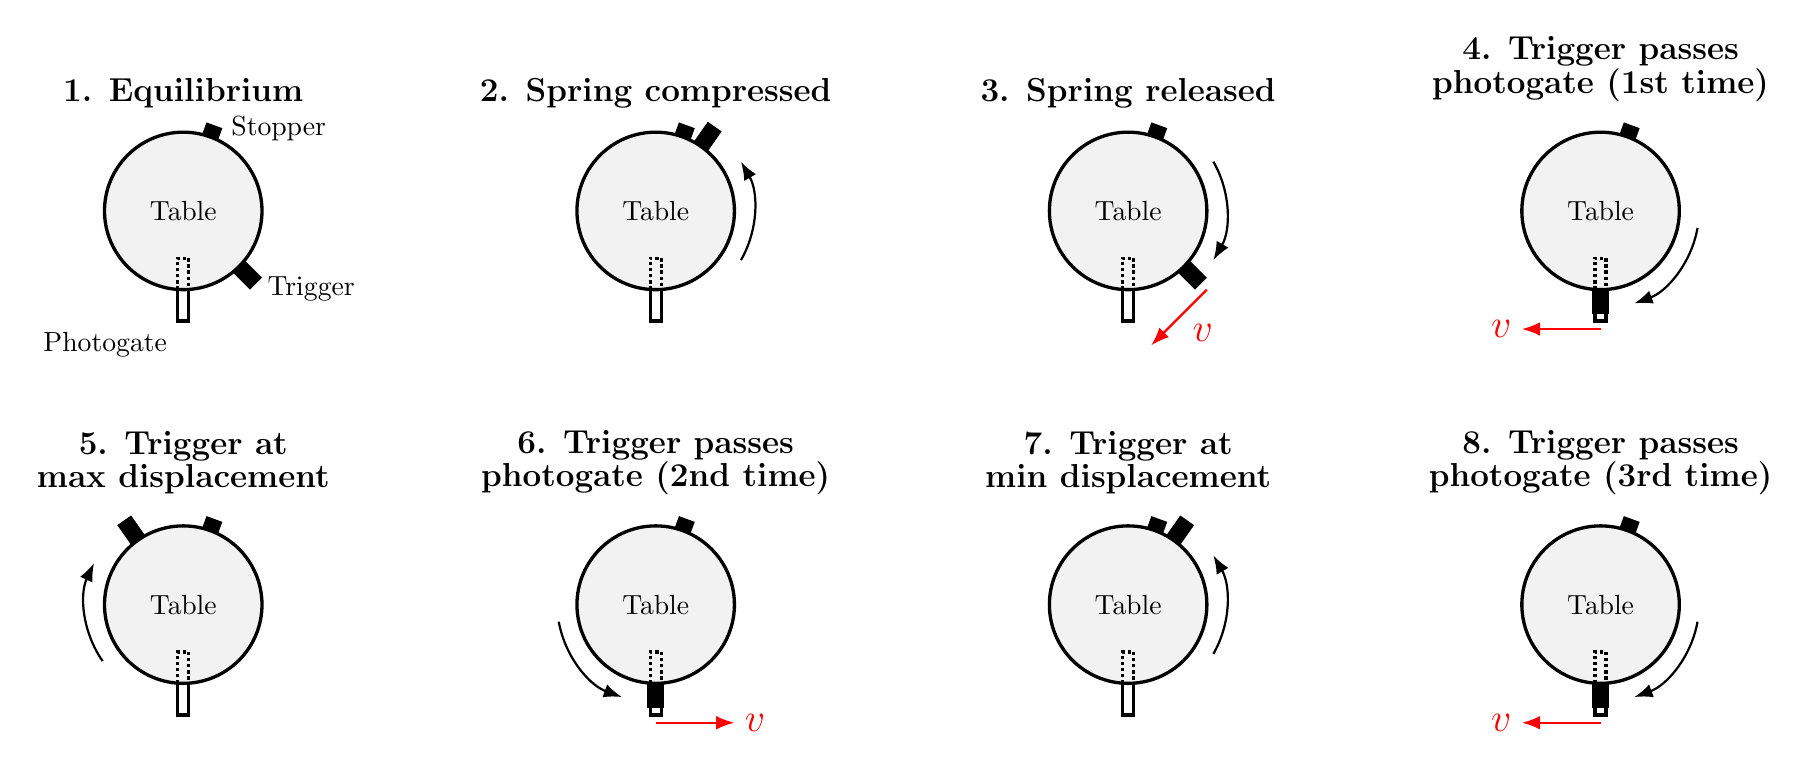
\begin{tikzpicture}
    %%% First row
    \draw (0,1.5) node {\large\bf 1. Equilibrium};
    \filldraw[color=black, fill=gray!10, very thick](0,0) node {Table} circle (1);
    \draw[color=black, very thick] (-0.07,-1.4) node[below left] {Photogate} rectangle (0.07,-1);
    \draw[color=black, very thick, densely dotted] (-0.07,-1) rectangle (0.07,-0.6);
    \draw[color=black, fill=black, rotate around={45:(0,0)}] (-0.1,-1.3) node[right, xshift=1mm] {Trigger} rectangle (0.1,-1);
    \draw[fill=black, rotate around={340:(0,0)}] (-0.1,1) rectangle (0.1,1.15) node[right] {Stopper};
    %
    \draw ({0+6},1.5) node {\large\bf 2. Spring compressed};
    \filldraw[color=black, fill=gray!10, very thick]({0+6},0) node {Table} circle (1);
    \draw[color=black, very thick] ({-0.07+6},-1.4) rectangle ({0.07+6},-1); % photogate
    \draw[color=black, very thick, densely dotted] ({-0.07+6},-1) rectangle ({0.07+6},-0.6);
    \draw[color=black, fill=black, rotate around={145:({0+6},0)}] ({-0.1+6},-1.3) rectangle ({0.1+6},-1); % trigger
    \draw[fill=black, rotate around={340:({0+6},0)}] ({-0.1+6},1) rectangle ({0.1+6},1.15); % stopper
    \draw[thick, -Latex] ({1.25*cos(30)+6}, {0-1.25*sin(30)}) arc (-30:30:1.25);
    %
    \draw ({0+12},1.5) node {\large\bf 3. Spring released};
    \filldraw[color=black, fill=gray!10, very thick]({0+12},0) node {Table} circle (1);
    \draw[color=black, very thick] ({-0.07+12},-1.4) rectangle ({0.07+12},-1); % photogate
    \draw[color=black, very thick, densely dotted] ({-0.07+12},-1) rectangle ({0.07+12},-0.6);
    \draw[color=black, fill=black, rotate around={45:({0+12},0)}] ({-0.1+12},-1.3) rectangle ({0.1+12},-1); % trigger
    \draw[fill=black, rotate around={340:({0+12},0)}] ({-0.1+12},1) rectangle ({0.1+12},1.15); % stopper
    \draw[thick, Latex-] ({1.25*cos(30)+12}, {-1.25*sin(30)}) arc (-30:30:1.25);
    \draw[thick, red, -Latex] (13, -1) -- node[midway,xshift=3mm,yshift=-2mm] {\Large $v$} ({13-cos(45)}, {-1-sin(45)});
    %
    \draw ({0+18},1.5) node[align=center, yshift=3mm] {\large\bf 4. Trigger passes\\ \large\bf photogate (1st time)};
    \filldraw[color=black, fill=gray!10, very thick]({0+18},0) node {Table} circle (1);
    \draw[color=black, very thick] ({-0.07+18},-1.4) rectangle ({0.07+18},-1); % photogate
    \draw[color=black, very thick, densely dotted] ({-0.07+18},-1) rectangle ({0.07+18},-0.6);
    \draw[color=black, fill=black, rotate around={0:({0+18},0)}] ({-0.1+18},-1.3) rectangle ({0.1+18},-1); % trigger
    \draw[fill=black, rotate around={340:({0+18},0)}] ({-0.1+18},1) rectangle ({0.1+18},1.15); % stopper
    \draw[thick, Latex-] ({1.25*cos(70)+18}, {-1.25*sin(70)}) arc (-70:-10:1.25);
    \draw[thick, red, -Latex] (18, -1.5) -- (17, -1.5) node[left] {\Large $v$};
    %
    %%% Second row
    \draw (0,{1.5-5}) node[align=center, yshift=3mm] {\large\bf 5. Trigger at\\ \large\bf max displacement};
    \filldraw[color=black, fill=gray!10, very thick](0,{0-5}) node {Table} circle (1);
    \draw[color=black, very thick] (-0.07,{-1.4-5}) rectangle (0.07,{-1-5}); % photogate
    \draw[color=black, very thick, densely dotted] (-0.07,{-1-5}) rectangle (0.07,{-0.6-5});
    \draw[color=black, fill=black, rotate around={215:(0,{0-5})}] (-0.1,{-1.3-5}) rectangle (0.1,{-1-5}); % trigger
    \draw[fill=black, rotate around={340:(0,{0-5})}] (-0.1,{1-5}) rectangle (0.1,{1.15-5}); % stopper
    \draw[thick, -Latex] ({1.25*cos(145)}, {-1.25*sin(145) - 5}) arc (-145:-205:1.25);
    %
    \draw ({0+6},{1.5-5}) node[align=center, yshift=3mm] {\large\bf 6. Trigger passes\\ \large\bf photogate (2nd time)};
    \filldraw[color=black, fill=gray!10, very thick]({0+6},{0-5}) node {Table} circle (1);
    \draw[color=black, very thick] ({-0.07+6},{-1.4-5}) rectangle ({0.07+6},{-1-5}); % photogate
    \draw[color=black, very thick, densely dotted] ({-0.07+6},{-1-5}) rectangle ({0.07+6},{-0.6-5});
    \draw[color=black, fill=black, rotate around={0:({0+6},{0-5})}] ({-0.1+6},{-1.3-5}) rectangle ({0.1+6},{-1-5}); % trigger
    \draw[fill=black, rotate around={340:({0+6},{0-5})}] ({-0.1+6},{1-5}) rectangle ({0.1+6},{1.15-5}); % stopper
    \draw[thick, -Latex] ({1.25*cos(170)+6}, {-1.25*sin(170)-5}) arc (-170:-110:1.25);
    \draw[thick, red, -Latex] (6, {-1.5-5}) -- (7, {-1.5-5}) node[right] {\Large $v$};
    %
    \draw ({0+12},{1.5-5}) node[align=center, yshift=3mm] {\large\bf 7. Trigger at\\ \large\bf min displacement};
    \filldraw[color=black, fill=gray!10, very thick]({0+12},{0-5}) node {Table} circle (1);
    \draw[color=black, very thick] ({-0.07+12},{-1.4-5}) rectangle ({0.07+12},{-1-5}); % photogate
    \draw[color=black, very thick, densely dotted] ({-0.07+12},{-1-5}) rectangle ({0.07+12},{-0.6-5});
    \draw[color=black, fill=black, rotate around={145:({0+12},{0-5})}] ({-0.1+12},{-1.3-5}) rectangle ({0.1+12},{-1-5}); % trigger
    \draw[fill=black, rotate around={340:({0+12},{0-5})}] ({-0.1+12},{1-5}) rectangle ({0.1+12},{1.15-5}); % stopper
    \draw[thick, -Latex] ({1.25*cos(30)+12}, {0-1.25*sin(30)-5}) arc (-30:30:1.25);
    %
    \draw ({0+18},{1.5-5}) node[align=center, yshift=3mm] {\large\bf 8. Trigger passes\\ \large\bf photogate (3rd time)};
    \filldraw[color=black, fill=gray!10, very thick]({0+18},{0-5}) node {Table} circle (1);
    \draw[color=black, very thick] ({-0.07+18},{-1.4-5}) rectangle ({0.07+18},{-1-5}); % photogate
    \draw[color=black, very thick, densely dotted] ({-0.07+18},{-1-5}) rectangle ({0.07+18},{-0.6-5});
    \draw[color=black, fill=black, rotate around={0:({0+18},{0-5})}] ({-0.1+18},{-1.3-5}) rectangle ({0.1+18},{-1-5}); % trigger
    \draw[fill=black, rotate around={340:({0+18},{0-5})}] ({-0.1+18},{1-5}) rectangle ({0.1+18},{1.15-5}); % stopper
    \draw[thick, Latex-] ({1.25*cos(70)+18}, {-1.25*sin(70)-5}) arc (-70:-10:1.25);
    \draw[thick, red, -Latex] (18, {-1.5-5}) -- (17, {-1.5-5}) node[left] {\Large $v$};
\end{tikzpicture}}

        Which number in the picture corresponds to when the photogate timer measures one period of oscillation, and why?
        \begin{solution}[1.5cm]
            One period is numbers 4 to 8, since the trigger returns to the photogate with $v$ pointed to the left.
        \end{solution}
    \end{parts}

    \filbreak
    \question
    In the second part of the lab, you will observe the oscillations of a spring loaded with a specific mass. However, you may notice that the spring will oscillate even when no mass is attached ($m=0$).
    \begin{parts}
        \part[\half] What is one reason why this can happen?
        \begin{solution}[1.5cm]
            The spring can oscillate under its own weight.
        \end{solution}

        \part[\half] What is one effect this could have on the experiment?
        \begin{solution}[1cm]
            It may be difficult to estimate the period of oscillation of an attached mass in isolation from the effect of the spring.
        \end{solution}
    \end{parts}
\end{prelab}

% LAB SECTION
\begin{labsection}

%%% Objectives
\begin{objective}
    In the first part of this laboratory exercise, you will measure the moment of inertia of three different objects about a specified rotational axis and verify the parallel axis theorem. In the second part, you will measure the oscillations of a mass on a spring to investigate Hooke’s Law.
\end{objective}

%%% Theory/background
\begin{theory}
    \subsection*{Moment of Inertia and the Parallel Axis Theorem}

    \begin{wrapfigure}{l}{0.3\linewidth}
        \centering
        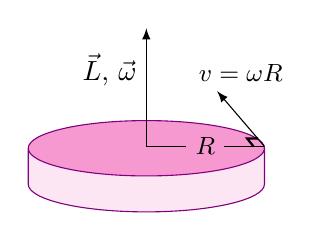
\begin{tikzpicture}
    \node[cylinder,
        draw=violet,
        cylinder uses custom fill, 
        cylinder body fill = magenta!10, 
        cylinder end fill = magenta!40,
        minimum width = 30mm,
        aspect = 3,
        shape border rotate = 90] (c) at (0,0) { };
    \draw[-latex] (0,0.5) -- (0,2) node[below left, yshift=-2mm] {$\vec{L}$, $\vec{\omega}$};
    \draw (0,0.5) -- node[midway, fill=magenta!40] {\small $R$} (1.5,0.5);
    \draw[-latex] (1.5,0.5) -- (0.9,1.2) node[above, xshift=3mm] {\small $v=\omega R$};
    \draw[thick] (1.42,0.6) -- (1.28,0.6) -- (1.36,0.5); 
\end{tikzpicture}
        \caption{A rotating solid disk. \label{fig: solid disk}}
    \end{wrapfigure}
    
    Consider a rigid body rotating about an axis, as in Fig.~\ref{fig: solid disk}. If the angular velocity is $\omega$, a point in the body at a perpendicular distance $r$ from the axis of rotation will move with linear speed $v=\omega r$. The total angular momentum $L$ of the rotating body points along the axis of rotation and is equal to
    %
    \begin{equation}\label{eq:angular momentum}
        L = \int_\text{body} rv~dm = \int_\text{body} r^2\omega~dm = \omega\int_\text{body} r^2~dm = I\omega,
    \end{equation}
    %
    where
    %
    \begin{equation}\label{eq:moment of inertia}
        I = \int_\text{body} r^2~dm
    \end{equation}
    %
    is called the {\bf moment of inertia} of the body about the axis of rotation. In the SI system of units, $I$ is expressed in units of kg~m$^2$.

    If the axis of rotation is chosen through the center of mass of the object, its moment of inertia about the center of mass is called $I_\text{CM}$. For example, for the solid disk of mass $M$ and radius $R$ shown in Fig.~\ref{fig: solid disk},
    \[
        I_\text{CM} = \frac{1}{2}MR^2.
    \]
    Table~\ref{tab: Icm} shows examples of $I_\text{CM}$ for other kinds of mass distributions.    

    \begin{table}[ht]
        \centering
        \renewcommand{\arraystretch}{1.5}
        \begin{tabular}{|c|c|c|}
        \hline
        {\bf Object}         & {\bf Rotational Axis}          & $\mathbf{I_\text{\bf CM}}$                   \\
        \hline
        Thin Ring            & Symmetry Axis    & $MR^2$ \\
        Thick Ring           & Symmetry Axis    & $\frac{1}{2}M\left(R_1^2 + R_2^2\right)$ \\
        Solid Disk           & Symmetry Axis    & $\frac{1}{2}MR^2$ \\
        Thin Spherical Shell & About a Diameter & $\frac{2}{3}MR^2$ \\
        Solid Sphere         & About a Diameter & $\frac{2}{5}MR^2$ \\
        \hline
        \end{tabular}
        \caption{Moments of inertia of several mass distributions. \label{tab: Icm}}
    \end{table}

    The {\bf parallel axis theorem}\footnote{Also called the Huygens–Steiner theorem, after Christiaan Huygens (1629-1695) and Jakob Steiner (1796-1863).} relates the moment of inertia about the center of mass, $I_\text{CM}$ to the moment of inertia $I$ about a parallel axis through some other point. The theorem states
    %
    \begin{equation}\label{eq:parallel axis theorem}
        I = I_\text{CM} + Md^2,
    \end{equation}
    %
    where $M$ is the body's mass and $d$ is the perpendicular distance between the two axes. This implies that $I_\text{CM}<I$ about any other parallel axis.

    \subsection*{Analogies between Rotational and Linear Motion}
    When working with rotational motion for rigid bodies, many of the equations are similar to the equations of motion for linear kinematics. For example, angular velocity is used in place of linear velocity, and the moment of inertia is used instead of the mass. Table~\ref{tab:linear rotation analogs} summarizes the correspondence between linear and rotational kinematics for rigid bodies.

    \begin{table}[ht]
        \centering
        \renewcommand{\arraystretch}{1.5}
        \begin{tabular}{|c|c|}
        \hline
        {\bf Linear Kinematics}                   & {\bf Rotational Kinematics}                    \\
        \hline
        $\text{Linear Velocity}=v$                & $\text{Angular Velocity}=\omega$               \\
        $\text{Mass}=M$                           & $\text{Moment of Inertia}=I$                   \\
        $\text{Linear Momentum}=p=Mv$             & $\text{Angular Momentum}=L=I\omega$            \\
        $\text{Kinetic Energy}=K=\frac{1}{2}Mv^2$ & $\text{Kinetic Energy}=K=\frac{1}{2}I\omega^2$ \\
        \hline
        \end{tabular}
        \caption{Analogies between linear and rotational motion. \label{tab:linear rotation analogs}}
    \end{table}
\end{theory}

\subsection*{Determining the Moment of Inertia of an Object}

\begin{wrapfigure}{r}{0.35\linewidth}
    \centering
    
\includegraphics[width=0.9\linewidth]{Lab 04: Moments of Inertia/torsion_table.png}
    \caption{Rotary table with torsion spring.\label{fig: torsion table}}
\end{wrapfigure}

The apparatus in Fig.~\ref{fig: torsion table} consists of a rotary table on which you can mount an object in order to measure its moment of inertia. A torsion spring restricts the motion of the table and provides a restoring torque $\tau$. If the table is rotated by an angle $\theta$, then the torque acting on it will be equal to
%
\begin{equation}\label{eq:hookes law}
    \tau = -\kappa\theta,
\end{equation}
%
where $\kappa$ is the torsion spring constant, analogous to the spring constant $k$ you are used to for compressed and stretched springs. The value of $\kappa$ must be measured.

If the sum of the moment of inertia of the table, $I_\text{tab}$, and that of the mounted object, $I_\text{obj}$, is equal to
$I_\text{obj} + I_\text{tab}$, then the table will perform a rotary oscillation with angular frequency
%
\begin{equation}\label{eq: table frequency}
    \omega = \sqrt{\frac{\kappa}{I_\text{obj} + I_\text{tab}}},
\end{equation}
%
which corresponds to a period of oscillation of
%
\begin{equation}\label{eq: table period}
    T = 2\pi\sqrt{\frac{I_\text{obj} + I_\text{tab}}{\kappa}}.
\end{equation}
%
Our two unknown parameters are $I_\text{tab}$ and $\kappa$. To determine their values, you will need to measure the oscillation period of the table alone ($T_\text{tab}$) and the period of the table plus object ($T_{\text{tab}+\text{obj}}$) when an object with known moment of inertia $I_\text{obj}$ is placed on the table. From eq.~\ref{eq: table period}, one finds that
%
\begin{align}
    T_\text{tab} &= 2\pi\sqrt{\frac{I_\text{tab}}{\kappa}} \label{eq: table period alone},
    \\
    T_{\text{tab} + \text{obj}} &= 2\pi\sqrt{\frac{I_\text{obj} + I_\text{tab}}{\kappa}} \label{eq: table-object period}.
\end{align}
%
To solve for $\kappa$, we square and add  eqs.~\ref{eq: table period alone} and \ref{eq: table-object period}, and also square and subtract, to get the following two equations:
%
\begin{align}
    (T_{\text{tab} + \text{obj}})^2 + (T_{\text{tab}})^2 &= 4\pi^2 \frac{2I_\text{tab} + I_\text{obj}}{\kappa} \label{eq: sys 1},
    \\
    (T_{\text{tab} + \text{obj}})^2 - (T_{\text{tab}})^2 &= 4\pi^2 \frac{I_\text{obj}}{\kappa} \label{eq: sys 2}.
\end{align}
%
Eq.~\ref{eq: sys 2} lets us isolate the torsion spring constant $\kappa$ in terms of known and measured quantities:
%
\begin{equation}\label{eq: torsion constant}
    \boxed{\kappa = 4\pi^2 \frac{I_\text{obj}}{(T_{\text{tab} + \text{obj}})^2 - (T_{\text{tab}})^2}}
\end{equation}
%
To find the unknown $I_\text{tab}$, divide eq.~\ref{eq: sys 1} by \ref{eq: sys 2}:
%
\begin{equation}\label{eq: sys 3}
    \frac{(T_{\text{tab} + \text{obj}})^2 + (T_{\text{tab}})^2}{(T_{\text{tab} + \text{obj}})^2 - (T_{\text{tab}})^2} = \frac{2I_\text{tab}}{I_\text{obj}} + 1,
\end{equation}
%
which we can then simplify and solve for our second unknown:
%
\begin{equation}\label{eq: moment table}
    \boxed{I_\text{tab} = I_\text{obj} \frac{(T_{\text{tab}})^2}{(T_{\text{tab}+\text{obj}})^2 - (T_{\text{tab}})^2}}
\end{equation}
%
If we have a body with a known moment of inertia, $I_\text{obj}$, eqs.~\ref{eq: torsion constant} and \ref{eq: moment table} will give us $\kappa$ and $I_\text{tab}$ with a few simple measurements. And once we know $\kappa$ and $I_\text{tab}$, we can find the moment of inertia $I_x$ of some other unknown object $x$ using the expression
%
\begin{equation}\label{eq: moment unknown}
    \boxed{I_x = I_\text{tab}\left[\left(\frac{T_{\text{tab}+x}}{T_\text{tab}}\right)^2 - 1\right]}\ ,
\end{equation}
%
as long as we also measure the period of oscillation of the table and the new object, $T_{\text{tab}+x}$.

\subsection*{Hooke's Law and Spiral Spring Oscillations}

It is often assumed that a long spiral spring will obey Hooke's law if it is not stretched too far. If the spring is hung vertically from a fixed support and a mass is attached to its free end, the mass can be made to oscillate vertically in a simple harmonic motion pattern by stretching and releasing it. The period of an oscillation is the time it takes the attached mass to return to its initial starting position. The period $T$ depends upon the attached mass $M$, the spring force constant $k$, and the spring mass $m$, and is given by
%
\begin{equation}\label{eq: spring period}
    T = 2\pi\sqrt{\frac{M + bm}{k}}.
\end{equation}
%
In eq.~\ref{eq: spring period}, $b$ is a dimensionless constant called the spring mass coefficient. You will calculate $b$ in this lab and compare your measurement to the theoretical value
%
\begin{equation}\label{eq: spring coefficient theoretical}
    b_\text{theory} = \frac{1}{3}.
\end{equation}
%
During the lab, you will measure $T$ for a variety of values of $M$. To make it easy to estimate $k$ given $T$ and $M$, square eq.~\ref{eq: spring period}:
%
\begin{equation}\label{eq: spring period squared}
    T^2 = \frac{4\pi^2}{k}M + \frac{4\pi^2}{k}bm.
\end{equation}
%
If we make a plot of $T^2$ versus $M$, eq.~\ref{eq: spring period squared} leads us to expect a linear relation of form
%
\begin{equation}\label{eq: spring period linear}
    y = (\text{slope})x + (\text{$y$-intercept}).
\end{equation}
%
You will plot the data in this manner and determine whether you obtain the expected linear relationship.

%%% Experiment
\newpage
\begin{experiment}

\subsection*{Moment of Inertial and Parallel Axis Theorem}
\subsubsection*{Procedure}

\begin{enumerate}
    \item Set up the rotary table and allow it to come to its equilibrium position. Make sure the tabletop is level by placing a level onto it and adjusting the apparatus' feet as needed.
    %
    \item Set the photogate timer to pendulum mode and arrange the photogate so the table's trigger (see Fig.~\ref{fig: rotary table}) passes through the photogate when the table rotates.

    {\centering
    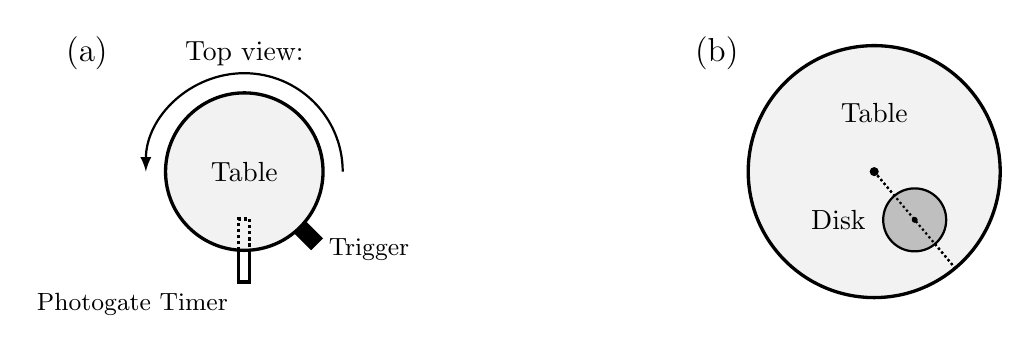
\begin{tikzpicture}
        \filldraw[color=black, fill=gray!10, very thick](0,0) node {Table} circle (1);
        \draw[color=black, very thick] (-0.07,-1.4) node[below left] {\small Photogate Timer} rectangle (0.07,-1);
        \draw[color=black, very thick, densely dotted] (-0.07,-1) rectangle (0.07,-0.6);
        \draw[color=black, fill=black, rotate around={45:(0,0)}] (-0.1,-1.3) node[right, xshift=1mm] {\small Trigger} rectangle (0.1,-1);
        \draw[thick, -latex] (1.25, 0) arc (0:180:1.25);
        \draw (0,1.5) node {Top view:};
        \draw (-2, 1.5) node {\large (a)};
        %
        \draw[color=black, fill=gray!10, very thick] (8,0) circle (1.6);
        \draw[fill=black] (8,0) node[above, yshift=5mm] {Table} circle (0.05);
        \draw[thick, densely dotted] (8,0) -- ({8 + 1.6*sin(40)},{-1.6*cos(40)});
        \draw[thick, fill=gray!50] ({8 + 0.8*sin(40)},{-0.8*cos(40)}) circle (0.4);
        \draw[fill=black] ({8 + 0.8*sin(40)},{-0.8*cos(40)}) node[left, xshift=-5mm] {Disk} circle (0.03);
        \draw[thick, densely dotted] (8,0) -- ({8 + 1.6*sin(40)},{-1.6*cos(40)});
        \draw ({-2+8}, 1.5) node {\large (b)};
    \end{tikzpicture}
    \captionof{figure}{(a) view of rotary table, photogate timer, and trigger; (b) the table with the disk at an offset from the axis of rotation. \label{fig: rotary table}}}

    \item Wind the table either clockwise or counter-clockwise such that {\sl the trigger does not pass the timer while winding}. Stop when the table hits the block and cannot be turned any further.
    %
    \item Release the table. Count the number of times the trigger passes through the photogate before the timer stops counting. It should be three passes before the timer stops. The displayed time will be the period of one oscillation.
    %
    \item Measure the mass and inner and outer radii of the {\sl brass ring}. Record your values in Data Table~\ref{data: ipa meas} in the Postlab Exercises.
    %
    \item Measure the period of one oscillation {\sl of the table alone} ($T_\text{tab}$) five (5) times. Record your data in Data Table~\ref{data: ipa meas} in the Postlab Exercises.
    %
    \item After ensuring the brass ring is mounted securely with screws to the tabletop and is centered on the table's axis of rotation, measure the period of oscillation {\sl of the table/ring combination} ($T_{\text{tab}+\text{ring}}$ five (5) times. Record the data in Data Table~\ref{data: ipa meas}.
    %
    \item Measure the mass and radius of the solid disk, and record your measurements in Data Table~\ref{data: ipa meas}.
    %
    \item To measure the period of one oscillation for the table/disk combination, secure the disk at one of five equally spaced positions along the table radius, a distance $d$ from the table's axis of rotation (see Fig.~\ref{fig: rotary table}). Start at the center ($d=\qty{0.000}{\meter}$). The recommended positions are \qty{0.000}{\meter}, \qty{0.015}{\meter}, \qty{0.030}{\meter}, \qty{0.045}{\meter}, and \qty{0.060}{\meter}, using the spacing holes on the table.
    %
    \item For each of the five positions $d$, measure the period of oscillation five (5) times. Record your data in Data Table~\ref{data: pa data}.
\end{enumerate}

\subsection*{Hooke's Law and Spiral Spring Oscillations}

\subsubsection*{Introduction}

According to Hooke's law, the extension of a stretched spring $x$ from its equilibrium position should be proportional to the force $F$ exerted on the spring by an attached mass,
%
\begin{equation}\label{eq: hookes law}
    F = -kx,
\end{equation}
%
where $k$ is the {\sl force constant} of the spring (also called the {\sl spring constant}). 
You will test the validity of Hooke's law by making measurements of $x$ while incrementally increasing $M$. 
Then, you will measure the period of oscillation of several hanging masses to estimate the spring mass coefficient $b$ neeeded to account for the spring's own mass $m$, as described in eqs.~\ref{eq: spring period} and \ref{eq: spring coefficient theoretical}.

\subsubsection*{Procedure}

\begin{enumerate}
    \item Weigh the Slinky Jr.\texttrademark\ and mass holder to determine the mass of the spring/slinky system $m$. Record it in Data Table~\ref{data: hookes law} in the Postlab Exercises.
    %
    \item Mount the spring by clipping one end of it to the flat metal piece mounted to the stand.
    %
    \item For each of the attached masses $M$ listed in Data Table~\ref{data: hookes law}, calculate the force of gravity $F=Mg$, where $g=\qty{9.8}{\meter/\second^2}$. Record your calculations in Data Table~\ref{data: hookes law}.
    %
    \item Let the spring come to equilibrium. If possible, move the ruler/spring vertically so that the ruler's zero is at the bottom of the spring (or the bottom of the mass holder, if you prefer). Record the position of the spring’s bottom end -- i.e. its equilibrium length -- on the ruler.
    %
    \item Measure the change in the extension of the spring, $x$, as you attach different amounts of mass to the end of the spring. Keep in mind that the ``extension of the spring'' is the length of the spring extended beyond the spring's equilibrium length. Use masses of \qty{5}{\gram}, \qty{10}{\gram}, \qty{15}{\gram}, \qty{20}{\gram}, and \qty{25}{\gram}. Attach the masses gently. Record all results in Data Table~\ref{data: hookes law}.
    %
    \item For each of the five masses $M$, measure the period of ten (10) oscillations. You can set the spring and mass into motion by {\bf gently} stretching the mass \qty{15}{\centi\meter} to \qty{20}{\centi\meter} and then releasing it. The mass should not touch the floor or anything else as it moves. If you pulled the mass down, then one oscillation occurs every time the mass returns to the lowest part of its oscillation (its initial position). {\bf Divide the total time by 10 to get the average period of one oscillation.} Record the average period for each value of $M$ in Data Table~\ref{data: hookes law}.
\end{enumerate}

\end{experiment}

\end{labsection}

% POSTLAB SECTION
\begin{postlab}

    %%% Section on moment of inertia and parallel axis theoream
    \fullwidth{\subsection*{Moment of Inertia and the Parallel Axis Theorem (\pointsinrange{mipatheorem} points)}}

    \begingradingrange{mipatheorem}

    \filbreak
    \question[3] Fill in data from your measurements of the moment of inertia in Data Table~\ref{data: ipa meas} and test of the parallel axis theorem in Data Table~\ref{data: pa data}.

    \begin{center}
        \renewcommand{\arraystretch}{2}
        \captionsetup{font=normalsize}
        \captionof{data table}{Data for the moments of inertia. \label{data: ipa meas}}
        \begin{tabular}{lp{3cm}p{1cm}|p{2cm}|p{2cm}|p{2cm}|}
        \cline{4-6}
        {\bf Ring Measurements}              & & & Trial       & $T_\text{tab}$ [s] & $T_{\text{tab}+\text{ring}}$ [s]
        \\
        \cline{4-6}
        Ring mass [kg] =               & & & 1           &                    &                                  \\
        \cline{2-2}\cline{4-6}
        Inner radius $R_1\text{ [m]}=$ & & & 2           &                    &                                  \\
        \cline{2-2}\cline{4-6}
        Outer radius $R_2\text{ [m]}=$ & & & 3           &                    &                                  \\
        \cline{2-2}\cline{4-6}
        {\bf Disk Measurements}              & & & 4           &                    &                                  \\
        \cline{4-6}
        Disk mass [kg] =               & & & 5           &                    &                                  \\
        \cline{2-2}\cline{4-6}
        Disk radius $R\text{ [m]}=$    & & & Average [s] &                    &                                 \\
        \cline{2-2}\cline{4-6}
        \end{tabular}
    \end{center}
    
    \begin{center}
        % Generated the table using https://www.tablesgenerator.com/
        \renewcommand{\arraystretch}{2.25}
        \captionsetup{font=normalsize}
        \captionof{data table}{Data for parallel axis theorem. \label{data: pa data}}
        \begin{tabular}{|p{2.2cm}|p{2.2cm}|p{2.2cm}|p{2.2cm}|p{2.2cm}|p{2.2cm}|}
        \hline
        Distance [m]  & $d_{x_1}=0.000$ & $d_{x_2}=$ & $d_{x_3}=$ & $d_{x_4}=$ & $d_{x_5}=$
        \\
        \hline
        Trial         & \multicolumn{1}{|c|}{$T_{x_1}$ [s]} & \multicolumn{1}{|c|}{$T_{x_2}$ [s]}  & \multicolumn{1}{|c|}{$T_{x_3}$ [s]}  & \multicolumn{1}{|c|}{$T_{x_4}$ [s]}  & \multicolumn{1}{|c|}{$T_{x_5}$ [s]}
        \\
        \hline\hline
        1             &                               &            &            &            &       \\
        \hline
        2             &                               &            &            &            &       \\
        \hline
        3             &                               &            &            &            &       \\
        \hline
        4             &                               &            &            &            &       \\
        \hline
        5             &                               &            &            &            &       \\
        \hline\hline
        Average [s] &                               &            &            &            &      
        \\
        \hline
        \end{tabular}
    \end{center}

    \newpage
    Next, calculate all values in Data Table~\ref{data: moments data}. For values of the measured periods, use the average values from Data Tables \ref{data: ipa meas} and \ref{data: pa data}. Write the formula for each quantity (except for $I_{x_2}$ to $I_{x_5}$) and the uncertainty. Remember to include units! You do not have to show your calculations.

    \begin{center}
    % Generated the table using https://www.tablesgenerator.com/
    \renewcommand{\arraystretch}{2.35}
    \captionsetup{font=normalsize}
    \captionof{data table}{Calculation of moments of inertia. \label{data: moments data}}
    \begin{tabular}{|p{8cm}|p{7cm}|}
    \hline
    Formula:                                    & \multirow{2}{7cm}{Theoretical value of the moment of inertia of the brass ring (Table~\ref{tab: Icm}). Note: we consider it a thick (and heavy) ring.}               
    \\
    \cline{1-1}
    $I_\text{ring}=$                             &                                                                                                                                            \\
    \cline{1-2}
    Formula:                                    & \multirow{2}{7cm}{Spring constant of the table, eq.~\ref{eq: torsion constant}, where $I_\text{obj}=I_\text{ring}$ and $T_{\text{tab}+\text{obj}}=T_{\text{tab}+\text{ring}}$.}
    \\
    \cline{1-1}
    $\kappa=$                                         &                                               \\
    \cline{1-2}
    Formula:                                    & \multirow{2}{7cm}{Calculated moment of inertia of the table, eq.~\ref{eq: moment table}, where $I_\text{obj}=I_\text{ring}$.}                           \\
    \cline{1-1}
    $I_\text{table}=$                            &                                               \\
    \cline{1-2}
    Formula:                                    & \multirow{2}{7cm}{Theoretical value of the moment of inertia of the brass disk (Table~\ref{tab: Icm}).}                                              \\
    \cline{1-1}
    $I_\text{disk}=$                             &                                               \\
    \cline{1-2}
    Formula:                                    & \multirow{2}{7cm}{Calculated moment of inertia when the brass disk is placed at $d_1$. Use eq. \ref{eq: moment unknown}, where $T_{\text{tab} + x}=T_{x_1}$.}
    \\
    \cline{1-1}
    $I_{x_1}=$                                   &                                               \\
    \hline
    $I_{x_2}=$                                   & Calculated moment of inertial when the brass disk is at $d_2$.                                                                     \\
    \hline
    $I_{x_3}=$                                   & Calculated moment of inertial when the brass disk is at $d_3$.                                                                     \\
    \hline
    $I_{x_4}=$                                   & Calculated moment of inertial when the brass disk is at $d_4$.                                                                     \\
    \hline
    $I_{x_5}=$                                   & Calculated moment of inertial when the brass disk is at $d_5$.                                                                     \\
    \hline
    $\text{Uncertainty}=|I_\text{disk}-I_{x_1}|=$ & Calculated uncertainty in the moment of inertia of the solid disk.
    \\
    \hline
    \end{tabular}
    \renewcommand{\arraystretch}{1}
    \end{center}

    \filbreak
    \question In Graph~\ref{graph: moment of inertia}:
    \begin{parts}
        \part[1] Plot $I_{x_i}$, the moment of inertia of the solid disk on the $y$-axis versus
        $d_{x_i}^2$, the {\sl square} of the distance between the center of the table and the center of the solid disk, on the $x$-axis.

        \part[\half] Include error bars on each data point. Each error bar should have the same length $|I_\text{disk}-I_{x_1}|$ from Data Table~\ref{data: moments data}.

        \part[\half] Add a title to the plot, label the axes, and include units.
    \end{parts}

    \begin{center}
        \captionsetup{font=normalsize}
        \captionof{graph}{Plot of $I_{x_i}$ versus $d_{x_i}^2$. \label{graph: moment of inertia}}
        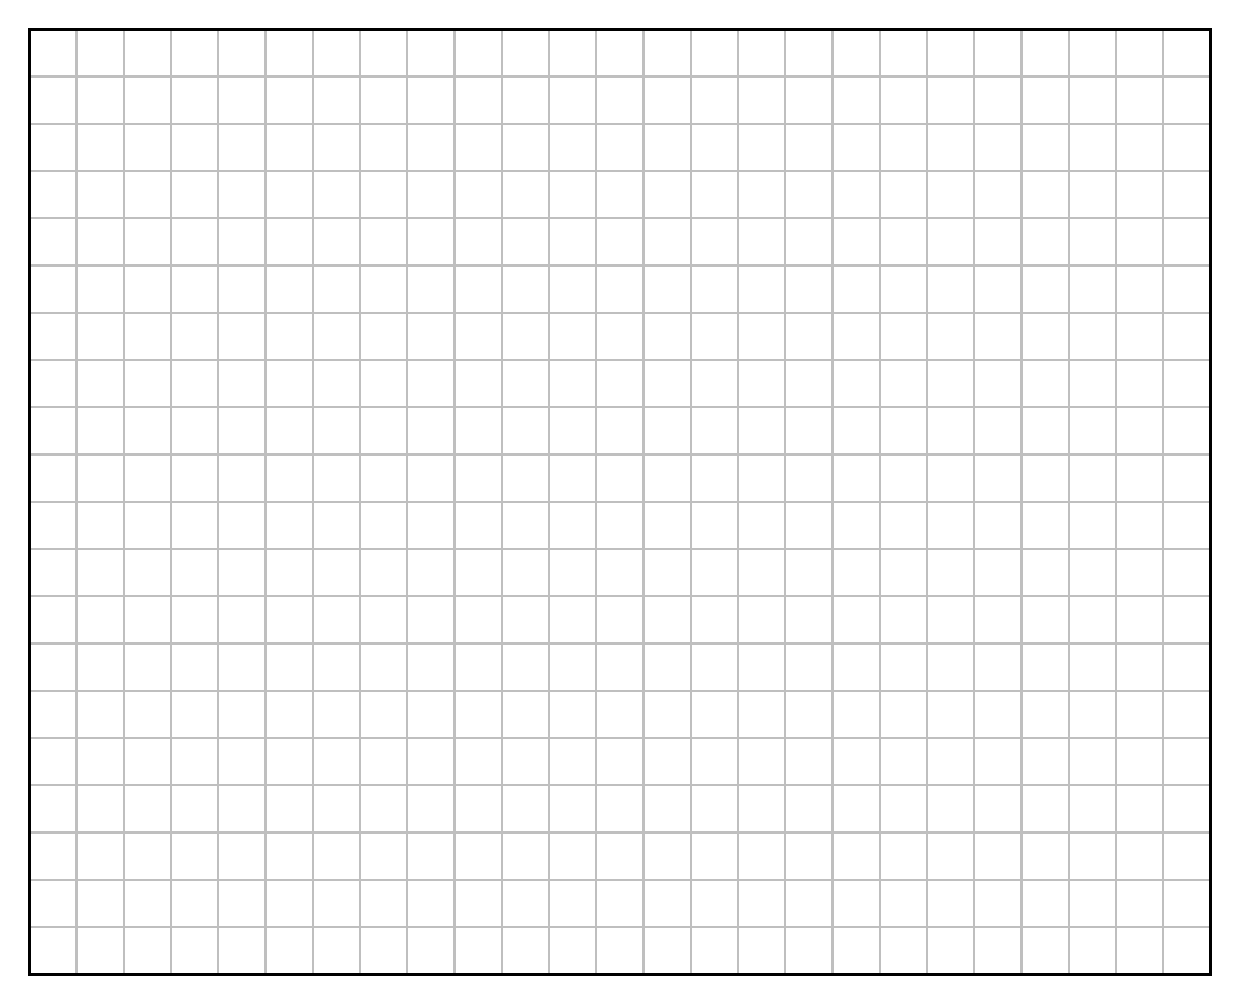
\begin{tikzpicture}
            % Define dimensions
            \def\gridwidth{25}
            \def\gridheight{20}
            \def\spacing{0.6}
            % Draw grid paper on the left
            \begin{scope}[xshift=0cm,yshift=0cm]
                % Major grid lines (thicker)
                \foreach \x in {0,1,...,\gridwidth}
                    \draw[gray!50,thick] (\x*\spacing,0) -- (\x*\spacing,\gridheight*\spacing);
                \foreach \y in {0,1,...,\gridheight}
                    \draw[gray!50, thick] (0,\y*\spacing) -- (\gridwidth*\spacing,\y*\spacing);
                \draw[black, very thick] (0,0) rectangle (\gridwidth*\spacing,\gridheight*\spacing);
            \end{scope}
        \end{tikzpicture}
    \end{center}

    \filbreak
    \question\label{q: exp fit}
    \begin{parts}
        \part[\half] In the plot, draw a best-fit straight line for your data. It need not go through the origin.

        \part[\half] Find the $y$-intercept of your best-fit line and circle it on the graph. Then circle two points on your best fit line, $(x_1,y_1)$ and $(x_2,y_2)$ and compute the slope. Write both values below:
        %
        \begin{flalign*}
            \\
            b_\text{exp} = y - \text{intercept} &= &&
            \\
            \\
            m_\text{exp} = \text{slope} = \frac{\Delta y}{\Delta x} = \frac{y_2-y_1}{x_2-x_1} &= &&
            \\
        \end{flalign*}
    \end{parts}

    \filbreak
    \question[1]\label{q: theory fit}
    If you take the parallel axis theorem
    \[
        I = Md^2 + I_\text{CM}
    \]
    and you plot $I$ versus $d^2$ ($y$ vs $x$), the data should be linear. Given that the equation for a line is $y=mx+b$, where $m$ is the slope and $b$ is the $y$-intercept, what variables in the parallel axis theorem correspond to $m$ and $b$?
    %
    \begin{flalign*}
        \\
        m_\text{theory} = \text{slope} &= &&
        \\
        \\
        b_\text{theory} = \text{intercept} &= &&
        \\
    \end{flalign*}

    \filbreak
    \question[2]
    Using your answers to questions \ref{q: exp fit} and \ref{q: theory fit}, how much do your measured values for the slope and $y$-intercept differ from the theoretical valeus? Remember to include units.{\color{red} I think this should say .... instead}
    %
    \begin{flalign*}
        \\
        |m_\text{theory} - m_\text{exp}| &= &&
        \\
        \\
        |b_\text{theory} - b_\text{exp}| &= &&
        \\
    \end{flalign*}

    \filbreak
    \question
    Name two sources of experimental error. Give a reason as to how each source of error would affect your values of the moment of inertia.
    %
    \begin{parts}
        \part[\half] First source of error:
        \begin{solution}[2cm]
            
        \end{solution}

        \part[\half] Second source of error:
        \begin{solution}[2cm]
            
        \end{solution}
    \end{parts}
    \endgradingrange{mipatheorem}

    %%% Section on Hooke's Law and spiral spring oscillations
    \fullwidth{\subsection*{Hooke's Law and Spiral Spring Oscillations (\pointsinrange{hlspiralspring} points)}}

    \begingradingrange{hlspiralspring}

    Add your measurements into Data Table~\ref{data: hookes law} below:

    \begin{center}
    \renewcommand{\arraystretch}{2}
    \captionsetup{font=normalsize}
    \captionof{data table}{Hooke's Law and Spiral Spring measurements. \label{data: hookes law}}
    \begin{tabular}{|p{4.25cm}|p{3cm}|p{2.2cm}|p{2.2cm}|p{2.2cm}|}
        \hline
        \multicolumn{2}{l}{$m=\text{mass of spring [kg]}=$}   & \multicolumn{1}{l}{}  & \multicolumn{2}{l}{}  \\
        \cline{2-2}
        \multicolumn{5}{l}{}                                                                                           \\
        \hline
        \rowcolor{gray!20}
        $M=\text{attached mass}$ [kg] & $\text{Force}=Mg$ [N] & Extension [m] & Period [s] & $\text{Period}^2$ [s$^2$] \\
        \hline
        0.005                         &                       &               &            &                           \\
        \hline
        0.010                         &                       &               &            &                           \\
        \hline
        0.015                         &                       &               &            &                           \\
        \hline
        0.020                         &                       &               &            &                           \\
        \hline
        0.025                         &                       &               &            &
        \\
        \hline
        \end{tabular}
    \end{center}

    \filbreak
    \question
    \begin{parts}
        \part[1] Plot the {\bf force} of gravity versus {\bf extension} ($y$ vs. $x$) in Graph~\ref{graph: hookes law} using the data from Data Table~\ref{data: hookes law}.

        \part[\half] Include a plot title, axis labels, and units.

        \part[\half] Draw a best-fit straight line through the data points.
    \end{parts}
    %
    \begin{center}
        \captionsetup{font=normalsize}
        \captionof{graph}{Force of gravity versus spring extension. \label{graph: hookes law}}
        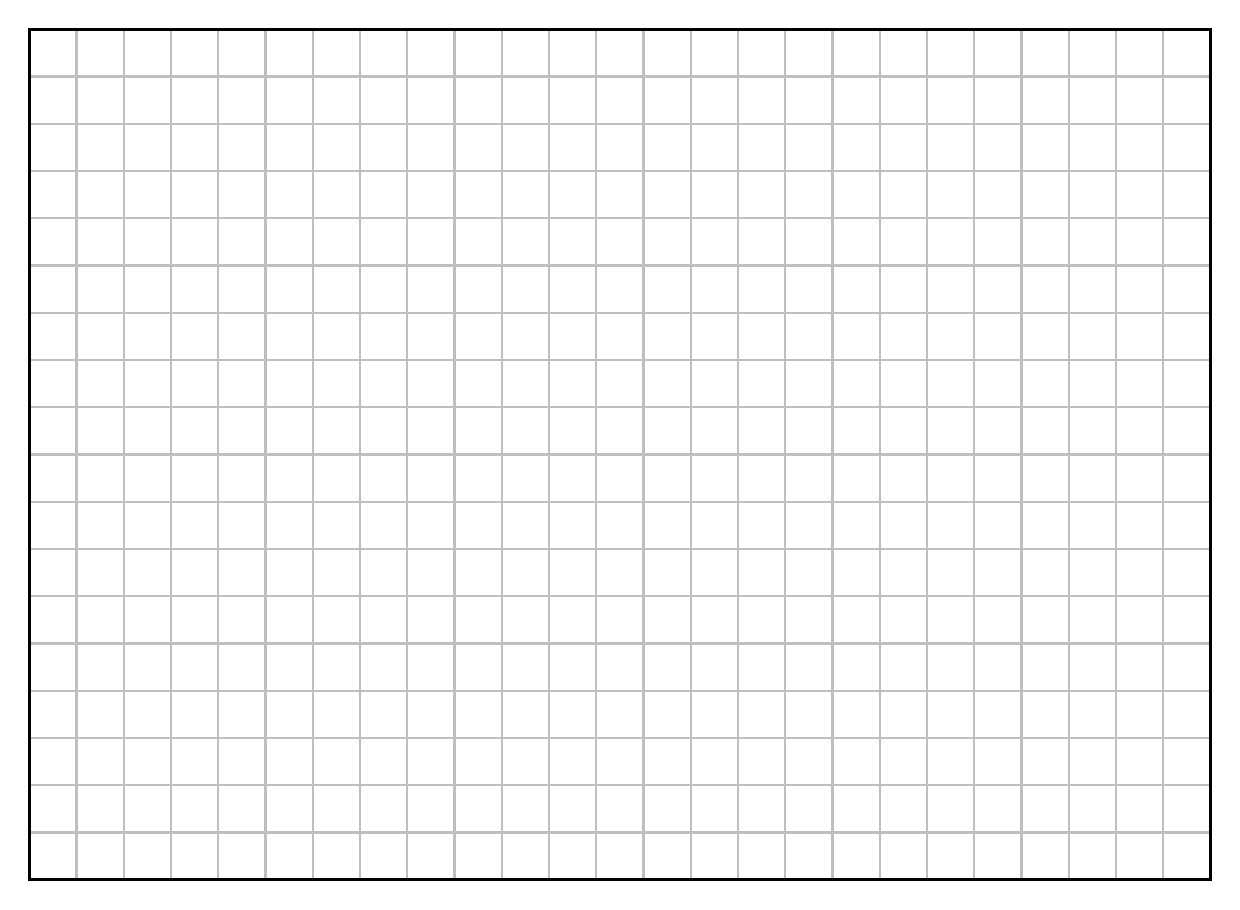
\begin{tikzpicture}
            % Define dimensions
            \def\gridwidth{25}
            \def\gridheight{18}
            \def\spacing{0.6}
            % Draw grid paper on the left
            \begin{scope}[xshift=0cm,yshift=0cm]
                % Major grid lines (thicker)
                \foreach \x in {0,1,...,\gridwidth}
                    \draw[gray!50,thick] (\x*\spacing,0) -- (\x*\spacing,\gridheight*\spacing);
                \foreach \y in {0,1,...,\gridheight}
                    \draw[gray!50, thick] (0,\y*\spacing) -- (\gridwidth*\spacing,\y*\spacing);
                \draw[black, very thick] (0,0) rectangle (\gridwidth*\spacing,\gridheight*\spacing);
            \end{scope}
        \end{tikzpicture}
    \end{center}

    \filbreak
    \question[1] Based on the best-fit straight line, does your data agree with Hooke's Law? Explain why.
    \begin{solution}[2cm]
        The student should explain that force depends linearly on the extension.
    \end{solution}

    \filbreak
    \question[1] \label{q: hookes slope}
    As in question~\ref{q: exp fit}, calculate the slope of the best-fit straight line. Circle two points $(x_1,y_1)$ and $(x_2,y_2)$ on the line that you will use to compute the slope, and use it to find the spring constant, $k_\text{Hooke}$. Don't forget units!
    %
    \begin{flalign*}
        k_\text{Hooke} &= \text{slope} = \frac{\Delta y}{\Delta x} = \frac{y_2-y_1}{x_2-x_1} = &&
    \end{flalign*}
    %
    \begin{solution}[1cm]
        Student should indicate the points used and report $k$ in N/m.
    \end{solution}

    \filbreak
    \question If we were to plot $T^2$ along the $y$-axis and $M$ along the $x$-axis:
    \begin{parts}
        \part[\half] What would be an equation for the theoretical value of the slope, $m_\text{theory}$, remembering that $y=mx+b$ is the equation for a line?
        \begin{solution}[2cm]
            
        \end{solution}

        \part[\half] What would be an equation for the theoretical value of the $y$-intercept, $b_\text{theory}$?
        \begin{solution}[2cm]
            
        \end{solution}
    \end{parts}

    \filbreak
    \question Using your data for $\text{Period}^2$ and the attached mass $M$ from Data Table~\ref{data: hookes law}:
    \begin{parts}
        \part[\half] Plot $\text{Period}^2$ versus attached mass, i.e., $T^2$ vs $M$, in Graph~\ref{graph: p2 vs m}.

        \part[\half] Draw a best-fit straight line through the data, and include a title, axis labels, and units.

    \end{parts}
    %
    \begin{center}
        \captionsetup{font=normalsize}
        \captionof{graph}{Period squared versus mass. \label{graph: p2 vs m}}
        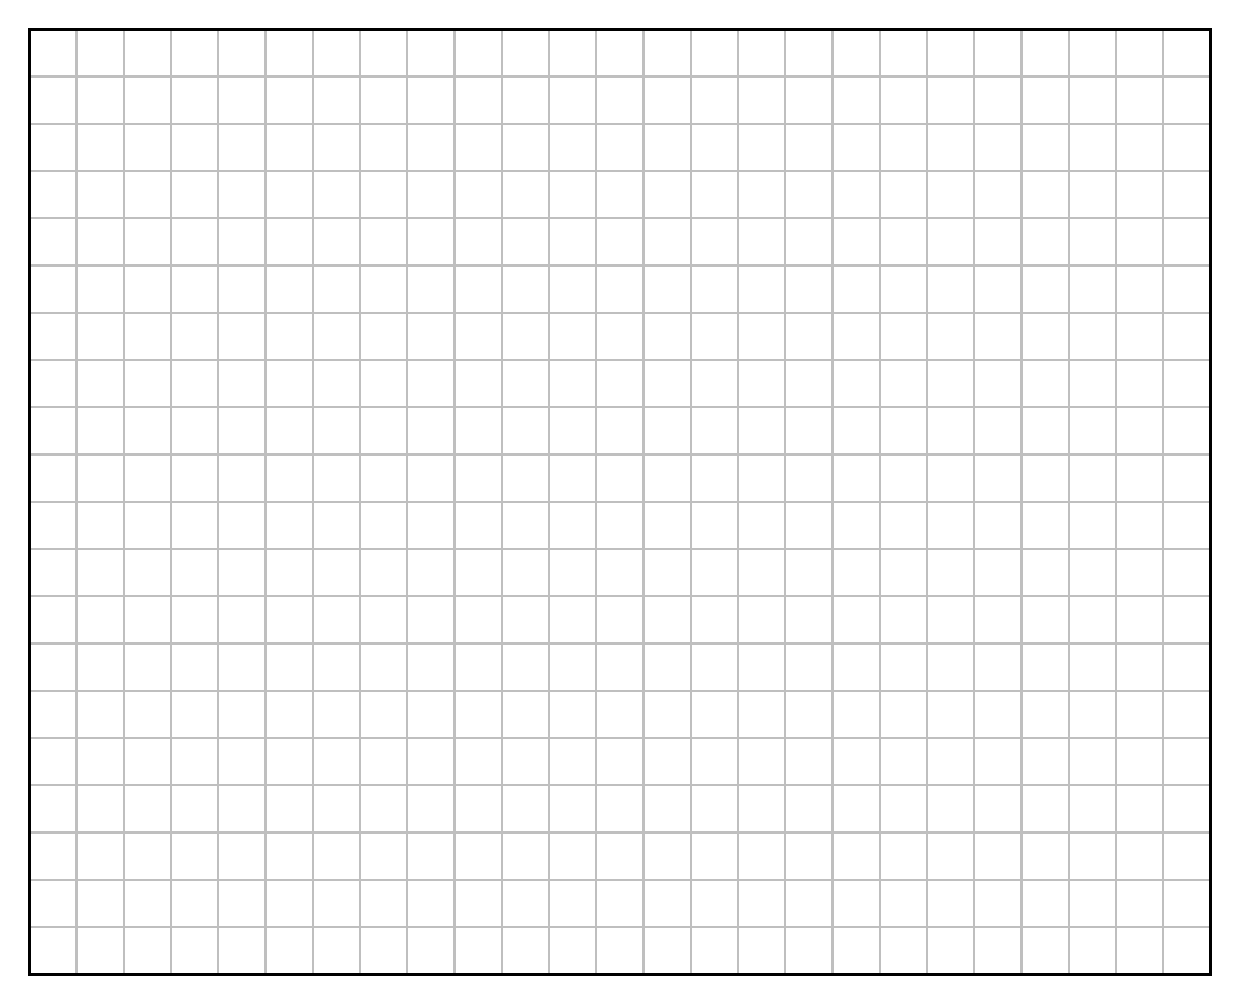
\begin{tikzpicture}
            % Define dimensions
            \def\gridwidth{25}
            \def\gridheight{20}
            \def\spacing{0.6}
            % Draw grid paper on the left
            \begin{scope}[xshift=0cm,yshift=0cm]
                % Major grid lines (thicker)
                \foreach \x in {0,1,...,\gridwidth}
                    \draw[gray!50,thick] (\x*\spacing,0) -- (\x*\spacing,\gridheight*\spacing);
                \foreach \y in {0,1,...,\gridheight}
                    \draw[gray!50, thick] (0,\y*\spacing) -- (\gridwidth*\spacing,\y*\spacing);
                \draw[black, very thick] (0,0) rectangle (\gridwidth*\spacing,\gridheight*\spacing);
            \end{scope}
        \end{tikzpicture}
    \end{center}

    \filbreak
    \question[1] \label{q: spring constant}
    Calculate the slope of the best-fit straight line. Circle two points on the line, $(x_1,y_1)$ and $(x_2,y_2)$. Setting the measured value of the slope to the equation you found in question \ref{q: hookes slope}, find the spring constant $k_\text{harm}$:
    %
    \begin{flalign*}
        \\
        m_\text{exp} = \text{slope} = \frac{\Delta y}{\Delta x} = \frac{y_2-y_1}{x_2-x_1} &= m_\text{theory} &&
        \\
        \\
        k_\text{harm} &= &&
    \end{flalign*}

    \filbreak
    \question[1] \label{q: spring coefficient}
    Find and circle the $y$-intercept of the best-fit straight line. Setting the measured value of the intercept to the equation you derived in question~\ref{q: hookes slope}, find the spring mass coefficient $b$. Use the spring constant $k$ you computed in question~\ref{q: spring constant}.
    % 
    \textcolor{red}{using $b_{exp}$ and $b_{theory}$ for y-int might confuse students since there are trying to find the spring mass coefficent which is also labeled b}
    \begin{flalign*}
        \\
        b_\text{exp} = \text{intercept} = b_\text{theory} &= &&
        \\
    \end{flalign*}

    \filbreak
    \question[1] Suppose that if the effective spring mass, $bm$, is less than 10\% of the smallest attached mass, $M=\qty{0.005}{kg}$, then we can say the spring mass is negligible. Based on the value of $b$ found in question~\ref{q: spring coefficient}, is the spring mass negligible? That is, do you find that
    \[
        \frac{bm}{M} \leq 0.1?
    \]
    \begin{solution}[2cm]   
    \end{solution}

    \filbreak
    \question Check whether the spring constants $k$ calcuated in questions \ref{q: hookes slope} and \ref{q: spring constant} are comparable in two steps:
    \begin{parts}
        \part[\half] Find the difference between the two $k$ values, including units:
        %
        \begin{flalign*}
            |k_\text{Hooke}-k_\text{harm}| &= &&
        \end{flalign*}
        %
        \begin{solution}[1cm]
            Students should report the differences in units of N/m.
        \end{solution}

        \part[\half] Suppose we assume the $k$ measurements are consistent if they differ by less than 10\% of the smaller of the two values. Is it the case that
        \[
            \frac{|k_\text{Hooke}-k_\text{harm}|}{k_\text{smaller}} \leq 0.1?
        \]
    \end{parts}

    \endgradingrange{hlspiralspring}

\end{postlab}

\end{document}